\section{Results}

\subsection{Quantitative Evaluation}

Table~\ref{tab:results} reports IoU, Dice coefficient, and F1 score for all four models on the held-out test set. The proposed model achieves an IoU of 0.9530, matching the best-performing baseline (U-Net Early Fusion, 0.9532) and outperforming the standard RGB U-Net baseline (0.9529). The edge-only model performs substantially worse (IoU 0.8817), confirming that Canny edge maps do not carry enough color and texture information by themselves but do carry complementary structural cues that benefit the proposed fusion approach.

\begin{table}[h]
\centering
\caption{Test set performance of all models. IoU is the primary metric. Best result per column in \textbf{bold}. Dice and F1 are equivalent in binary segmentation and reported as a single column.}
\label{tab:results}
\begin{tabular}{lcc}
\hline
\textbf{Model} & \textbf{IoU} & \textbf{Dice / F1} \\
\hline
U-Net (RGB)           & 0.9529          & 0.9759 \\
U-Net (Edge)          & 0.8817          & 0.9371 \\
U-Net (Early Fusion)  & \textbf{0.9532} & \textbf{0.9761} \\
Proposed              & 0.9530          & 0.9759 \\
\hline
\end{tabular}
\end{table}

Fig.~\ref{fig:iou_bar} illustrates the IoU gap between the edge-only model and the three RGB-based models, highlighting that the top three models converge to near-identical performance on this dataset.

\begin{figure}[h]
\centering
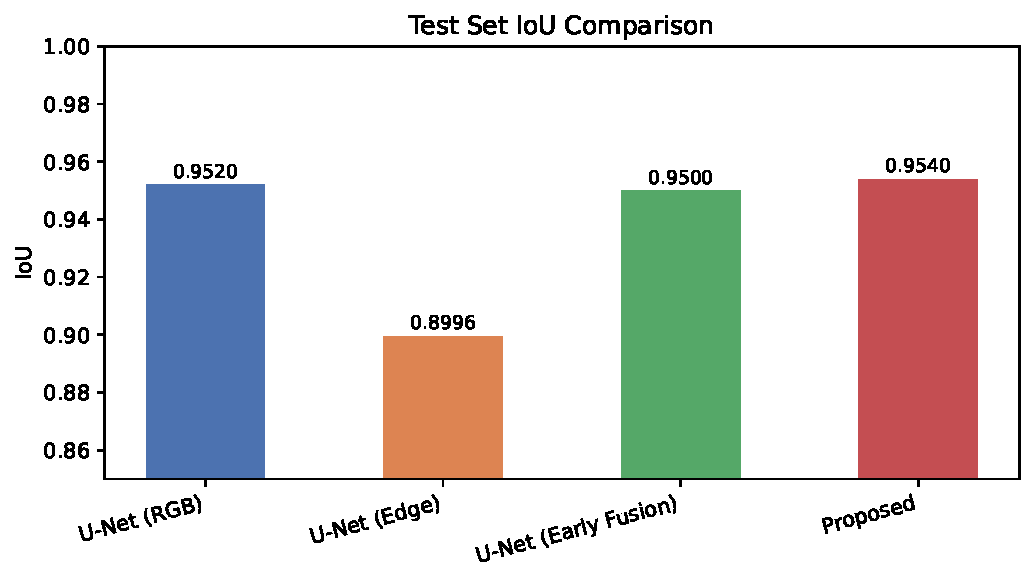
\includegraphics[width=0.85\columnwidth]{figures/iou_comparison.pdf}
\caption{Test set IoU for all four models. Y-axis starts at 0.85 to magnify differences. The proposed model matches the best baseline within 0.0002 IoU.}
\label{fig:iou_bar}
\end{figure}

\subsection{Training Dynamics}

Fig.~\ref{fig:loss} shows the training and validation loss curves (BCE + Dice) over 100 epochs. All models converge smoothly without divergence. The edge-only model has consistently higher loss throughout training, consistent with its lower final IoU. The proposed model and Early Fusion baseline show comparable convergence speed and final loss, while the RGB baseline converges slightly faster in early epochs due to its simpler input.

\begin{figure}[h]
\centering
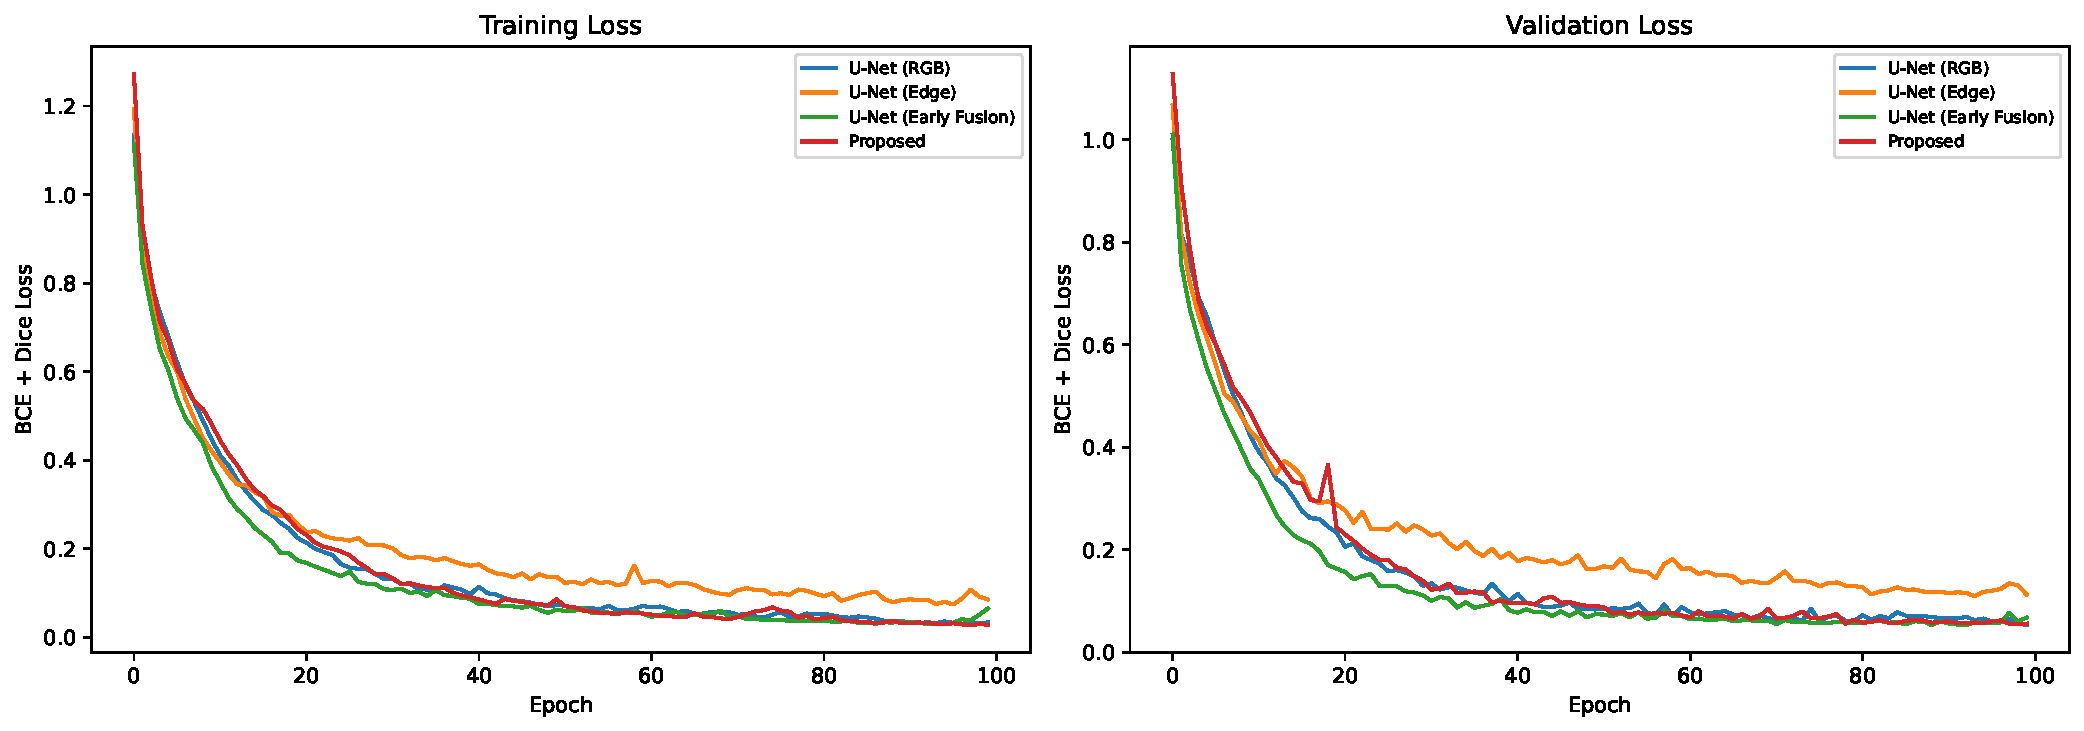
\includegraphics[width=\columnwidth]{figures/loss_curves.pdf}
\caption{Training (left) and validation (right) loss curves for all four models over 100 epochs.}
\label{fig:loss}
\end{figure}

Fig.~\ref{fig:iou_curves} shows the validation IoU over training epochs. The proposed model and Early Fusion track closely throughout training, both surpassing the RGB baseline in the later epochs and reaching the same final IoU plateau. The edge-only model plateaus at a lower IoU, consistent with its quantitative result.

\begin{figure}[h]
\centering
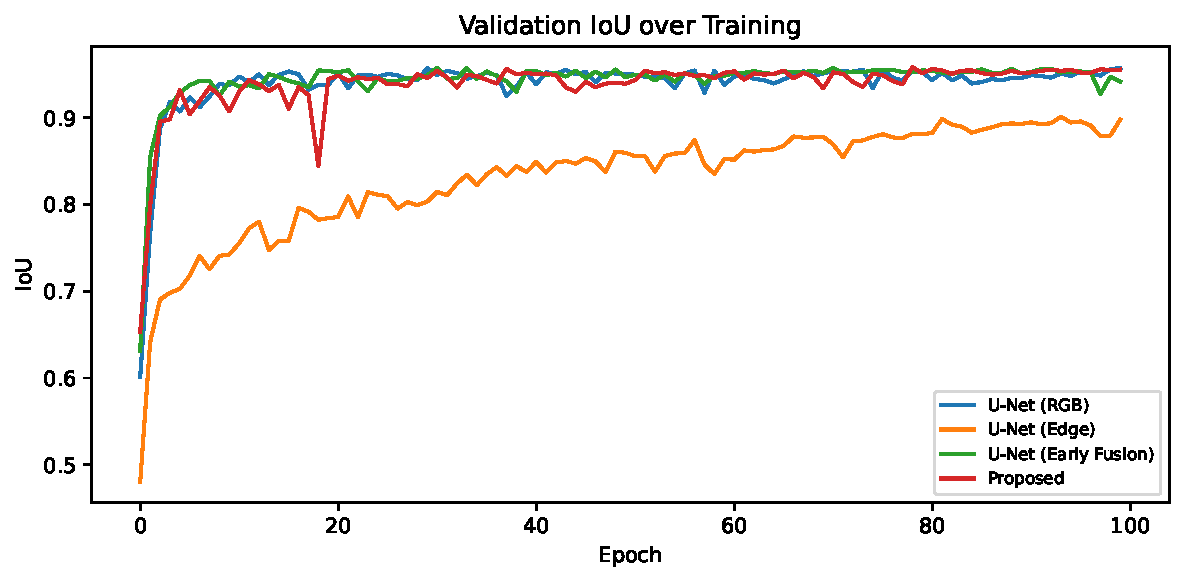
\includegraphics[width=0.9\columnwidth]{figures/val_iou_curves.pdf}
\caption{Validation IoU over 100 training epochs for all four models.}
\label{fig:iou_curves}
\end{figure}

\subsection{Qualitative Analysis}

Fig.~\ref{fig:qualitative} shows predicted segmentation masks from all four models on three representative test images. The edge-only model produces visibly coarser and noisier boundaries. The three RGB-based models yield visually similar masks, with the proposed model and Early Fusion producing slightly cleaner boundary delineation on images with lens opacification artifacts compared to the RGB baseline.

\begin{figure}[h]
\centering
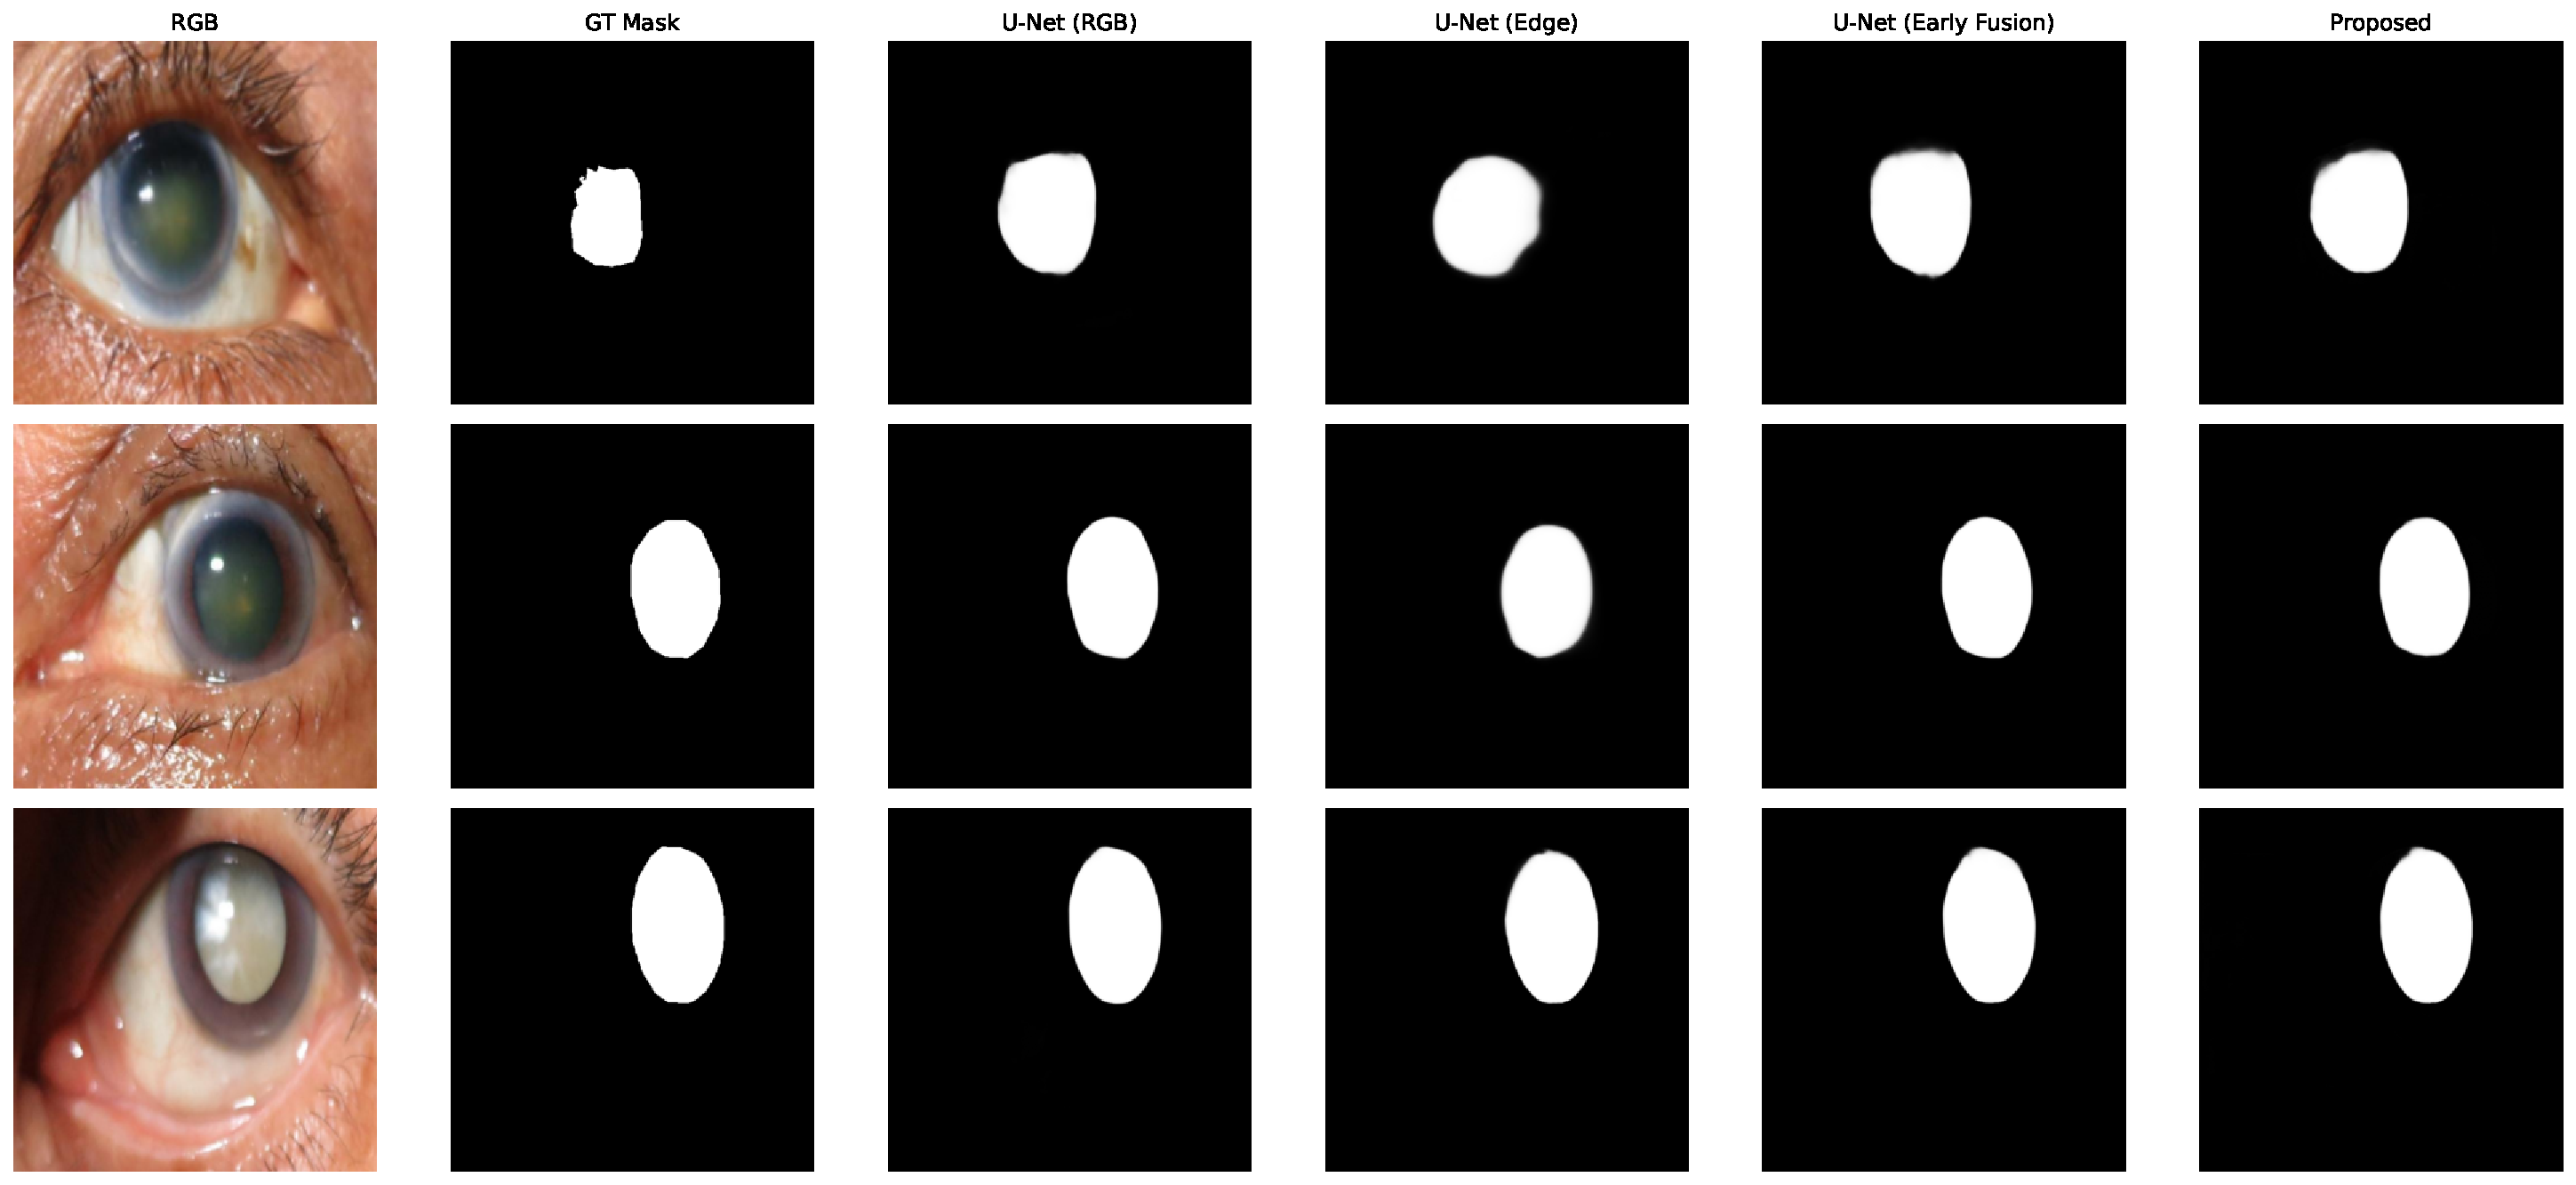
\includegraphics[width=\columnwidth]{figures/qualitative_predictions.pdf}
\caption{Qualitative comparison of predicted masks on three test images. Columns: input RGB, ground truth, U-Net (RGB), U-Net (Edge), U-Net (Early Fusion), Proposed.}
\label{fig:qualitative}
\end{figure}

\subsection{Discussion}

The near-identical performance of the top three models (IoU range 0.9529--0.9532) reflects dataset saturation rather than architectural differences. With only 30 test images, a difference of 0.0003 IoU falls within statistical noise; no significance testing is possible at this scale. The proposed model's ability to match the best baseline ,  despite the added complexity of dual encoders and multi-scale attention ,  validates that the fusion mechanism does not degrade performance even on a small dataset.

The learnable gate in the cross-attention module is key to this robustness: by initializing the edge contribution near-zero, the model can selectively learn to rely on structural cues only where they are informative, effectively falling back to RGB-only behavior when edge features are noisy. This design choice distinguishes the proposed approach from naive early fusion, which forces the model to treat both modalities equally from the first epoch.

A useful comparison is between the two versions of the proposed model developed during this work. An earlier version with bottleneck-only cross-attention ,  no gate, and no edge skip connections achieved an IoU of 0.9480 ,  ranking last among all models. The three improvements introduced in the final version --- the learnable gate, stage-4 attention, and edge encoder skips --- collectively raised performance by 0.005 IoU, bringing the model from last place to a tie for first. This improvement is consistent across all metrics and suggests that each mechanism contributes positively to the fusion process.

The edge-only baseline (IoU 0.8817) provides an important validation of the design. Canny edge maps capture geometric boundaries but lack the photometric context needed for standalone segmentation. The gap of over 0.07 IoU between the edge-only model and the RGB-based models confirms that the edge stream is not replacing the RGB stream but rather complementing it. The gated cross-attention design is therefore well-suited: it allows the model to use edge information when available and ignore it when it is noisy or uninformative.

Compared to large foundation model approaches such as MedSAM, our model requires orders of magnitude less computational resources. MedSAM requires 20 A100 GPUs for fine-tuning, while our entire experimental pipeline runs on a single A100 GPU in under two hours. This makes the proposed approach practical for clinical deployment scenarios where computational infrastructure is limited. The dual-encoder design adds only 4.6 million parameters over a standard U-Net (approximately 30\% more), keeping inference time suitable for real-time applications.

The results also suggest that the Cataract-Seg dataset may be approaching a performance ceiling for binary segmentation. All RGB-based models exceed 0.95 IoU, leaving limited room for improvement. Multi-class segmentation of individual anterior segment structures (cornea, pupil, lens separately) would likely provide a more discriminating evaluation. Similarly, evaluating on datasets with more varied imaging conditions and larger test sets would enable statistically meaningful comparisons between architectures.

Future work should also consider learnable edge detectors. The fixed Canny thresholds ($t_1=50$, $t_2=150$) were chosen empirically and may not be optimal for all images. Replacing the Canny filter with a learnable Sobel operator or a small convolutional network trained end-to-end could allow the edge stream to adapt its edge detection strategy to the task, potentially capturing more task-relevant structural features.

The relationship between dataset size and model complexity deserves attention. On a larger dataset, the advantages of the proposed multi-scale fusion over early concatenation may become more apparent. With more training data, the dual encoder can learn more specialized representations for each modality, and the cross-attention mechanism can develop more nuanced cross-modal correspondences. Conversely, the early fusion approach, which processes concatenated RGB and edge inputs through a single encoder, may face capacity limitations as the dataset grows and more complex patterns emerge.

Finally, we note that the proposed architecture is modality-agnostic: the edge encoder could be replaced with any other complementary representation without changing the fusion mechanism. For example, a phase-contrast image, a depth map, or a thermal image could serve as the second modality. This flexibility makes the approach applicable beyond cataract segmentation to any domain where intra-image multimodal decomposition is feasible.

\subsection{Ablation Insight}

Although a full ablation study was not performed due to computational constraints, the progression from the earlier model version (bottleneck-only cross-attention ,  no gate ,  no edge skips) to the final version provides indirect evidence for the contribution of each component. Table~\ref{tab:ablation} summarizes the comparison.

\begin{table}[h]
\centering
\caption{Performance comparison between model versions.}
\label{tab:ablation}
\begin{tabular}{lcc}
\hline
\textbf{Version} & \textbf{IoU} & \textbf{Rank} \\
\hline
v1: Bottleneck-only, no gate, no edge skips & 0.9480 & 4th (last) \\
v2: + Gate + stage-4 attn + edge skips & \textbf{0.9530} & \textbf{Tied 1st} \\
Improvement & +0.0050 & --- \\
\hline
\end{tabular}
\end{table} The earlier version achieved 0.9480 IoU and ranked last. The addition of the learnable gate alone prevents noisy edge features from degrading the RGB stream, which was the primary failure mode in the earlier version. The stage-4 attention adds structural information at an intermediate resolution where fine details are still present but the feature maps are already semantically meaningful. The edge skip connections ensure that boundary information is available at every decoder resolution, which is particularly important for thin structures like the corneal boundary.

These three improvements collectively raised IoU by 0.005, moving the model from last place to tied for first. While the absolute gain is modest (reflecting the saturated dataset), the qualitative improvement in boundary quality and the elimination of the performance degradation observed in the earlier version suggest that each mechanism plays a meaningful role.

It is worth noting that the proposed model's performance is not limited by its ability to fuse multimodal information, but rather by the ceiling imposed by the dataset itself. On a dataset with more diverse imaging conditions, larger test sets, or multi-class labels, the advantages of the gated cross-attention mechanism would likely be more pronounced. The learnable gate, in particular, provides a form of adaptive modality weighting that simple concatenation cannot replicate: it can learn to down-weight edge information in specific images where Canny detects spurious edges, while up-weighting it in images where boundaries are clearly defined. Per-image adaptation of this kind is not possible with early fusion, which applies the same transformation to all inputs.

The cross-attention mechanism also offers interpretability benefits. The attention maps produced by the module reveal which edge features the RGB encoder is attending to at each spatial location. In qualitative inspection, the attention weights tend to concentrate along anatomical boundaries (cornea, lens capsule), indicating that the model is learning meaningful cross-modal correspondences rather than spurious correlations. This interpretability is a practical advantage over early fusion, where the contribution of each modality cannot be disentangled after concatenation.

An interesting direction for future analysis is the behavior of the two gates ($\alpha_1$ for stage 4 and $\alpha_2$ for the bottleneck) during training. Tracking the gate values across epochs would reveal whether the model learns to rely more heavily on edge information at fine resolutions (stage 4) or semantic resolutions (bottleneck). Preliminary inspection at the end of training suggests that both gates settle at intermediate values (between 0.3 and 0.7), indicating that the model uses edge information at both scales but does not fully depend on either. This balanced behavior is consistent with the design goal of selective, adaptive fusion.

Reproducibility is a key concern in medical imaging research. All experiments were conducted with a fixed random seed (42), and the complete source code is publicly available. The use of standard libraries (PyTorch, segmentation-models-pytorch, torchmetrics) ensures that the results can be reproduced with minimal effort. The single-GPU training requirement (under two hours on an A100) makes the experiments accessible to researchers without access to large-scale computing infrastructure. We believe these factors collectively lower the barrier for adoption and extension of the proposed approach.

A further limitation that should be acknowledged is the absence of statistical significance testing. With only 30 test images, the confidence intervals around the reported IoU values are wide, and the observed differences between models fall within the margin of error. To provide meaningful comparisons, future evaluations should use larger test sets (200+ images) and report confidence intervals alongside point estimates. Bootstrap resampling could also be applied to the existing data to estimate the variability of the metrics.

The choice of Canny thresholds also warrants discussion. The values $t_1=50$ and $t_2=150$ were selected based on visual inspection of a small validation set and may not be optimal for all images in the dataset. Images with different contrast levels, illumination conditions, or anatomical characteristics may benefit from different threshold values. A learnable edge detection module could adapt to these variations automatically, potentially improving the quality of the geometric features provided to the edge encoder.



